\cleardoublepage



\chapter{Résultats - Discussion}

Nous ayons pu terminer le projet dans les temps seulement, même si celui-ci est aujourd'hui fonctionnel, il persiste encore certains problèmes.
Concernant tout d'abord les applications mobiles, certaines contraintes imposés par les systèmes d'exploitations nous ont empêches de construire une application qui marche sur n'importe quel téléphone.
\\





%%%%%%%%%%%%%%%%%%%%%%%%%%%%%%%%%%%%%%%%%%%%%%%%%%%%%%%%%%%%%%%%%%%%%%%%%%%%%%%%%%%%%%%%%%%%%%%%%%%%
%%%%%%%%%%%%%%%%%%%%%%%%%%%%%%%%%%%%%%%%%%%%%%%%%%%%%%%%%%%%%%%%%%%%%%%%%%%%%%%%%%%%%%%%%%%%%%%%%%%%
%%%%%%%%%%%%%%%%%%%%%%%%%%%%%%%%%%%%%%%%%%%%%%%%%%%%%%%%%%%%%%%%%%%%%%%%%%%%%%%%%%%%%%%%%%%%%%%%%%%%
%%%%%%%%%%%%%%%%%%%%%%%%%%%%%%%%%%%%%%%%%%%%%%%%%%%%%%%%%%%%%%%%%%%%%%%%%%%%%%%%%%%%%%%%%%%%%%%%%%%%
%%%%%%%%%%%%%%%%%%%%%%%%%%%%%%%%%%%%%%%%%%%%%%%%%%%%%%%%%%%%%%%%%%%%%%%%%%%%%%%%%%%%%%%%%%%%%%%%%%%%

\section{Site web}

Concernant le site web, les résultats obtenus sont probants.
Néanmoins, plusieurs fonctionnalités auxquels nous avions pensé manquent.
\\



%%%%%%%%%%%%%%%%%%%%%%%%%%%%%%%%%%%%%%%%%%%%%%%%%%%%%%%%%%%%%%%%%%%%%%%%%%%%%%%%%%%%%%%%%%%%%%%%%%%%
%%%%%%%%%%%%%%%%%%%%%%%%%%%%%%%%%%%%%%%%%%%%%%%%%%%%%%%%%%%%%%%%%%%%%%%%%%%%%%%%%%%%%%%%%%%%%%%%%%%%
%%%%%%%%%%%%%%%%%%%%%%%%%%%%%%%%%%%%%%%%%%%%%%%%%%%%%%%%%%%%%%%%%%%%%%%%%%%%%%%%%%%%%%%%%%%%%%%%%%%%

\subsection{Les contacts}

%%%%%%%%%%%%%%%%%%%%%%%%%%%%%%%%%%%%%%%%%%%%%%%%%%%%%%%%%%%%%%%%%%%%%%%%%%%%%%%%%%%%%%%%%%%%%%%%%%%%

\subsubsection{Cahier des charges}

Notre cahier des charges requérait une gestion simple et transparente des contacts pour l'utilisateur.

Le téléchargement des contacts du compte Google couplé avec l'affichage de la liste des noms de ces contacts, permet à l'utilisateur d'envoyer des SMS très simplement sans avoir à spécifier le numéro de téléphone.
\\

%%%%%%%%%%%%%%%%%%%%%%%%%%%%%%%%%%%%%%%%%%%%%%%%%%%%%%%%%%%%%%%%%%%%%%%%%%%%%%%%%%%%%%%%%%%%%%%%%%%%

\subsubsection{Apple}

Par défaut sous Androïd les contacts du téléphone sont dupliqués sur le serveur Google grâce au compte associés au smartphone, et on peut y avoir accès depuis Gmail par exemple.
Sous iOS cette fonction existe mais n'est pas associé à Google : Apple utilise iCloud qui permet aux utilisateurs une synchronisation automatique des contacts sur tous les appareils Apple associés à l'adresse mail.
Ainsi par défaut il n'est pas possible d'accéder aux contacts de l'iPhone depuis le site web.

Contrairement à Google qui effectue ses authentifications avec OAuth, Apple ne propose pas d'API permettant l'authentification sur iCloud.
La solution trouvée a donc été de synchroniser les contacts de l'iPhone avec un compte Google, au détriment de la synchronisation d'iCloud.
\\

%%%%%%%%%%%%%%%%%%%%%%%%%%%%%%%%%%%%%%%%%%%%%%%%%%%%%%%%%%%%%%%%%%%%%%%%%%%%%%%%%%%%%%%%%%%%%%%%%%%%

\subsubsection{Filtre}

Dans notre site web nous avons filtré la liste des contacts à ceux présents dans notre carnet d'adresses et en nous limitant aux numéros de téléphone portable (06.xx.xx.xx.xx ou 07.xx.xx.xx.xx).

Or il est possible de recevoir des SMS venant de numéro "courts" (8.xx.xx), de numéros de téléphone fixe, ou bien encore de contacts non présents dans nos contacts.

Notre version actuelle ne permet pas de résoudre ce problème.
Une solution serait d'ajouter un filtre sur la page web et enregistrer tous les contacts ainsi que ceux non présents dans Google.
\\



%%%%%%%%%%%%%%%%%%%%%%%%%%%%%%%%%%%%%%%%%%%%%%%%%%%%%%%%%%%%%%%%%%%%%%%%%%%%%%%%%%%%%%%%%%%%%%%%%%%%
%%%%%%%%%%%%%%%%%%%%%%%%%%%%%%%%%%%%%%%%%%%%%%%%%%%%%%%%%%%%%%%%%%%%%%%%%%%%%%%%%%%%%%%%%%%%%%%%%%%%
%%%%%%%%%%%%%%%%%%%%%%%%%%%%%%%%%%%%%%%%%%%%%%%%%%%%%%%%%%%%%%%%%%%%%%%%%%%%%%%%%%%%%%%%%%%%%%%%%%%%

\subsection{Anciens SMS}

Lorsque l'on se déconnecte du site web toutes les conversations sont supprimées du serveur en raison de la politique de sécurisé que nous avons voulu garder.
Nous avons pensé apporter une amélioration à notre site web, qui aurait pour objectif de télécharger les anciens messages échangés avec un contact.
Ces SMS transiteraient aussi par le protocole XMPP, soit un par un, soit sous forme de liste selon les performances et la taille maximale des messages XMPP.
\\





%%%%%%%%%%%%%%%%%%%%%%%%%%%%%%%%%%%%%%%%%%%%%%%%%%%%%%%%%%%%%%%%%%%%%%%%%%%%%%%%%%%%%%%%%%%%%%%%%%%%
%%%%%%%%%%%%%%%%%%%%%%%%%%%%%%%%%%%%%%%%%%%%%%%%%%%%%%%%%%%%%%%%%%%%%%%%%%%%%%%%%%%%%%%%%%%%%%%%%%%%
%%%%%%%%%%%%%%%%%%%%%%%%%%%%%%%%%%%%%%%%%%%%%%%%%%%%%%%%%%%%%%%%%%%%%%%%%%%%%%%%%%%%%%%%%%%%%%%%%%%%
%%%%%%%%%%%%%%%%%%%%%%%%%%%%%%%%%%%%%%%%%%%%%%%%%%%%%%%%%%%%%%%%%%%%%%%%%%%%%%%%%%%%%%%%%%%%%%%%%%%%
%%%%%%%%%%%%%%%%%%%%%%%%%%%%%%%%%%%%%%%%%%%%%%%%%%%%%%%%%%%%%%%%%%%%%%%%%%%%%%%%%%%%%%%%%%%%%%%%%%%%

\section{Applications mobiles}

Au vu des des techniques employés, il nous parait peu probable de pouvoir publier aucune des
deux applications sur les "markets" officiels de Apple et Google.
\\



%%%%%%%%%%%%%%%%%%%%%%%%%%%%%%%%%%%%%%%%%%%%%%%%%%%%%%%%%%%%%%%%%%%%%%%%%%%%%%%%%%%%%%%%%%%%%%%%%%%%
%%%%%%%%%%%%%%%%%%%%%%%%%%%%%%%%%%%%%%%%%%%%%%%%%%%%%%%%%%%%%%%%%%%%%%%%%%%%%%%%%%%%%%%%%%%%%%%%%%%%
%%%%%%%%%%%%%%%%%%%%%%%%%%%%%%%%%%%%%%%%%%%%%%%%%%%%%%%%%%%%%%%%%%%%%%%%%%%%%%%%%%%%%%%%%%%%%%%%%%%%

\subsection{Androïd}

%%%%%%%%%%%%%%%%%%%%%%%%%%%%%%%%%%%%%%%%%%%%%%%%%%%%%%%%%%%%%%%%%%%%%%%%%%%%%%%%%%%%%%%%%%%%%%%%%%%%

\subsubsection{Problèmes rencontrés}

De nombreux problèmes sont venus troubler l'avancement du projet. Nous avons toujours essayer de les
résoudre de la manière la plus efficiente qui soit. Seulement, il nous est arrivé de bloquer sur des
parties pour lesquelles aucune solutions propres n'étaient réalisable. Nous avons alors du appliquer 
des manipulations qui empêcheront ce projet d'être un projet considéré comme stable dans un environnement
grand public.


\paragraph{Message Gtalk}

Ce problème concerne autant l'architecture iOS que Androïd. 

Le choix de prendre GTalk comme moyen de communication n'était pas sans conséquences. En effet, il nous
est apparu impossible d'avoir une gestion fine de GTalk.
\\


Lors de l'envoi d'un message XMPP d'un compte A vers un compte B, toutes les interfaces de connexions
de B recevront le message. GTalk ne fait malheureusement pas exception de plus dans notre cas, l'envoi
se fait d'un compte A vers le même compte A. En pratique cela revient à recevoir et traiter beaucoup de
message inutiles.
\\


Premièrement, en ce qui concerne le traitement, les applications étant connectés sur leur compte GTalk, 
le message envoyé sera immédiatement reçu par l'application. Celle-ci bien heureusement filtrera les 
messages qui ne lui sont pas destinés.

\begin{figure}[!h]
	\center
	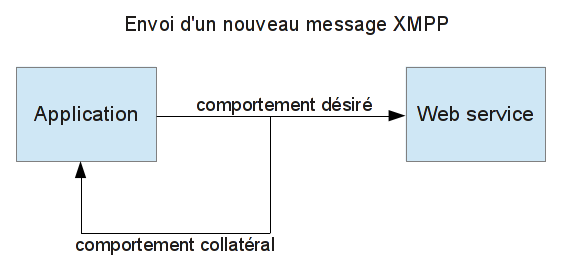
\includegraphics[width=12cm]{img/boucle-envoi-xmpp.png}
	\caption{Création d'une boucle lors de l'envoi d'un message XMPP}
	\label{boucle-envoi-xmpp}
\end{figure}

Comme le montre l'image \ref{boucle-envoi-xmpp}, une boucle se crée. Dans les faits, elle ne causera jamais de problème 
néanmoins c'est un comportement qui n'était pas désiré et qu'on aurait souhaitait évité.
\\


Deuxièmement, l'utilisation de GTalk était problématique. L'impossibilité de gérer finement GTalk fait que
tous les messages que nous envoyons, que ce soit depuis le téléphone ou bien depuis le site web étaient
aussi redirigés vers les outils utilisant GTalk.

En pratique, cela impliquait de recevoir des messages au format JSon sur plusieurs lieux indésirables.

\begin{figure}[!h]
	\center
	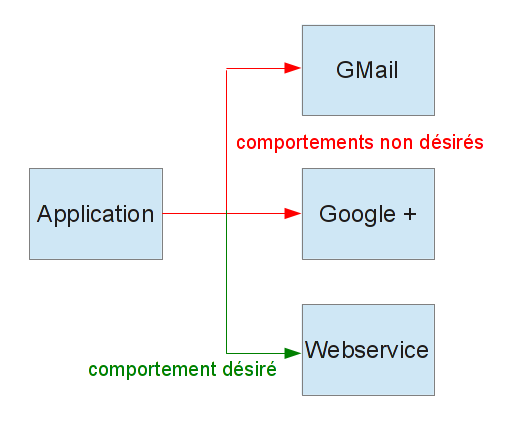
\includegraphics[width=10cm]{img/broadcast-xmpp.png}
	\caption{destinataires lors d'un envoi d'un message XMPP}
	\label{broadcast-xmpp}
\end{figure}

Comme le montre le schéma \ref{broadcast-xmpp}, lors de l'envoi d'un message XMPP originellement destiné uniquement
à une application ou au webservice, c'est tous l'environnement qui reçoit et affiche le nouveaux messages.
Le résultat est montré dans l'image \ref{message-xmpp-json-gmail}, un message XMPP au format JSon. 
	
\begin{figure}[!h]
	\center
	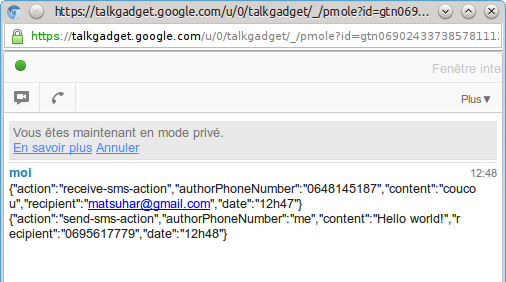
\includegraphics[width=10cm]{img/message-xmpp-json-gmail.png}
	\caption{message XMPP au format JSON reçu avec GTalk}
	\label{message-xmpp-json-gmail}
\end{figure}

%%%%%%%%%%%%%%%%%%%%%%%%%%%%%%%%%%%%%%%%%%%%%%%%%%%%%%%%%%%%%%%%%%%%%%%%%%%%%%%%%%%%%%%%%%%%%%%%%%%%

\paragraph{Limite des SMS}

Un autre soucis que nous avons rencontré sur la plateforme Androïd est la limite de SMS. Pour empêcher
les applications de spammer à la place d'un utilisateur, Androïd a mis en place une limite d'envoi de 
SMS pour une application. Toute application ne peut envoyer plus de 100 SMS par jours. Une fois la limite
atteinte, l'application est bridé. Chaque nouveau SMS envoyé doit alors faire l'objet d'une confirmation
par l'utilisateur ce qui rend le projet inutile car nous perdons l'avantage de pouvoir se passer du 
téléphone portable.

Malgré nos recherches sur le sujet, il s'est avéré impossible de modifier cette limite en passant par
des solutions réglementaires. La limite est défini dans la base de donnée système du système d'exploitation
qu'on ne peut modifier sans avoirs les droits Root.

Les droits Root correspondent simplement à avoir le droit de tout modifier sur son système avec les 
risques que cela comporte. Il faut savoir que pour obtenir ces droits, il faut rooter son téléphone.
Bien que rooter son téléphone est légal en soit, il comporte certains risques. Une mauvaise manipulation
peut engendrer des dommages sur le téléphone. De plus l'action en elle même n'est pas à la porté des 
débutants.
\\


Ces principales raisons font que notre application ne fonctionnera correctement que sur les téléphones
possédant les droits root. Cela implique que l'utilisateur devra être capable de manipuler son téléphone.

Pour pouvoir outrepasser ces contraintes, il est nécessaire de modifier le comportement par défaut du 
système. Nous avons utiliser un éditeur de bases de données SQLite avec lequel nous avons modifié une clé 
particulière. Il s'agit de la clé sms\_outgoing\_check\_max\_count que nous avons positionné à un nombre négatif
afin de ne plus avoir de limite d'envoi de message.

Cela modifié, nous sommes alors en mesure d'envoyer autant de messages que désiré. 
\\



%%%%%%%%%%%%%%%%%%%%%%%%%%%%%%%%%%%%%%%%%%%%%%%%%%%%%%%%%%%%%%%%%%%%%%%%%%%%%%%%%%%%%%%%%%%%%%%%%%%%
%%%%%%%%%%%%%%%%%%%%%%%%%%%%%%%%%%%%%%%%%%%%%%%%%%%%%%%%%%%%%%%%%%%%%%%%%%%%%%%%%%%%%%%%%%%%%%%%%%%%
%%%%%%%%%%%%%%%%%%%%%%%%%%%%%%%%%%%%%%%%%%%%%%%%%%%%%%%%%%%%%%%%%%%%%%%%%%%%%%%%%%%%%%%%%%%%%%%%%%%%

\subsection{iOS}

%%%%%%%%%%%%%%%%%%%%%%%%%%%%%%%%%%%%%%%%%%%%%%%%%%%%%%%%%%%%%%%%%%%%%%%%%%%%%%%%%%%%%%%%%%%%%%%%%%%%



\subsubsection{Les SMS}

- envoi du SMS : n'apparait pas dans les messages : ajout à la main dans la BDD ?

Impossible de lire les contacts...
\\
